\subsection{Salvataggio dataset}

\begin{figure}[H]
    \centering
    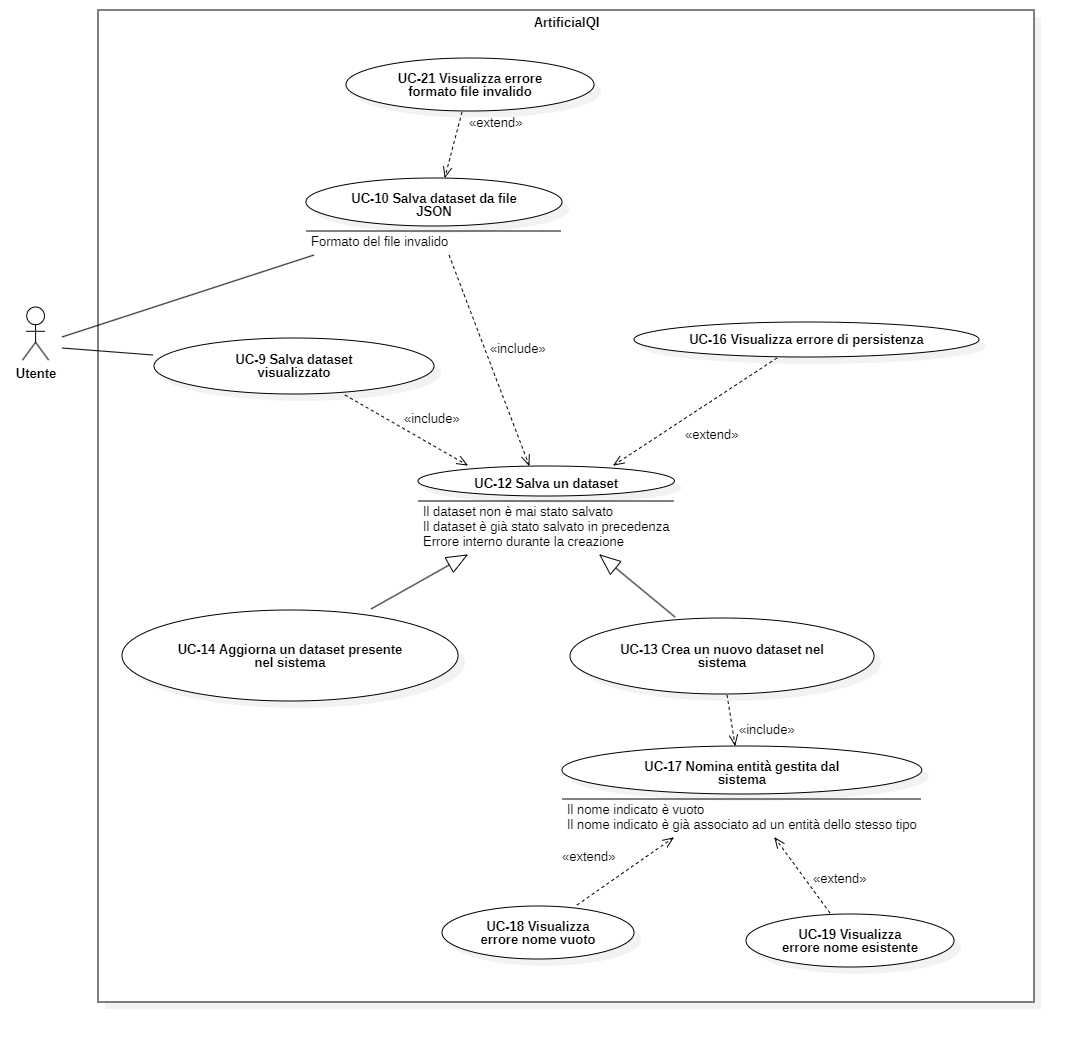
\includegraphics[scale=0.43]{Sezioni/UseCase/Immagini/SalvataggioDataset.png}
    \caption{Diagramma salvataggio dataset.}
\end{figure}

\begin{usecase}{UC-11}{Salva dataset visualizzato}
    \label{uc:UC-11}    
    
    \req{\hyperref[ru:RUO-3]{RUO-3}} 

    \pre{
        \item L'utente sta visualizzando una pagina del dataset da salvare \hyperref[uc:UC-1]{UC-1}
        \item Il dataset visualizzato non è vuoto
        \item Il dataset visualizzato non possiede una versione salvata o possiede una versione salvata non aggiornata
    }

    \post{
        \item Il dataset visualizzato viene salvato nel sistema
    }
    
    \actor{Utente}

    \subactors{}

    \trigger{L'utente vuole salvare il dataset visualizzato}
    
    \inc{\hyperref[uc:UC-12]{UC-12}}

    \base{}

    \scenario{
        \item L'utente richiede il salvataggio del dataset visualizzato
        \item Il sistema esegue il salvataggio seguendo \hyperref[uc:UC-12]{UC-12}
    }

    \subscenario{}
\end{usecase}

\begin{usecase}{UC-12}{Salva un dataset}
    \label{uc:UC-12}
    
    \req{}

    \pre{
        \item Il dataset ha delle modifiche da salvare
    }

    \post{
        \item Le modifiche vengono salvate
    }

    \actor{Utente}

    \subactors{}

    \trigger{Il sistema deve salvare un dataset}

    \inc{}

    \base{}

    \scenario{
        \item Il sistema verifica che il dataset da salvare sia stato già salvato in precedenza
    }
    
    \subscenario{
        \item [1.1] Errore interno durante la creazione:
        \begin{itemize}
            \item \hyperref[uc:UC-16]{UC-16}
        \end{itemize}
    }
\end{usecase}

\begin{usecase}{UC-13}{Creazione nuovo dataset nel sistema}
    \label{uc:UC-13}
    
    \req{} 

    \pre{
        \item Il dataset non è mai stato salvato
    }

    \post{
        \item Il dataset viene salvato 
    }
    
    \actor{Utente}

    \subactors{}

    \trigger{Il sistema deve salvare un nuovo dataset}

    \inc{\hyperref[uc:UC-17]{UC-17}}

    \base{\hyperref[uc:UC-12]{UC-12}}

    \scenario{
        \item Viene richiesta l'assegnazione di un nome per il nuovo dataset seguendo \hyperref[uc:UC-17]{UC-17}
        \item L'utente conferma la creazione di un nuovo dataset
        \item Il sistema salva il dataset
    }

    \subscenario{
        \item [1.1] L'utente annulla la creazione:
        \begin{itemize}
            \item Il sistema interrompe l'operazione
        \end{itemize}
    }

\end{usecase}

\begin{usecase}{UC-14}{Aggiorna dataset presente nel sistema}
    \label{uc:UC-14}
    
    \req{} 

    \pre{
        \item Il dataset è stato già salvato in precedenza 
    }

    \post{
        \item La versione del dataset salvata viene aggiornata
    }

    \actor{Utente}
    
    \subactors{}

    \trigger{Il sistema deve aggiornare la versione salvata di un dataset}

    \inc{}

    \base{\hyperref[uc:UC-12]{UC-12}}

    \scenario{
        \item Il sistema verifica la presenza di test associati alla versione del dataset da aggiornare
        \item Il sistema aggiorna la versione salvata
        \item L'utente viene avvisato del corretto aggiornamento
    }

    \subscenario{
        \item[1.1] Il dataset da aggiornare è associato all'esecuzione di uno o più test:
        \begin{itemize}
            \item Il sistema chiede all'utente se vuole annullare l'operazione
            \item L'utente conferma l'annullamento
            \item Il sistema interrompe l'operazione
        \end{itemize}
        \item[2.1] Il dataset da aggiornare è associato all'esecuzione di uno o più test:
        \begin{itemize}
            \item Il sistema chiede all'utente se copiare il dataset e aggiornare la copia \hyperref[uc:UC-24]{UC-24}
            \item L'utente conferma la copia
            \item Il sistema copia il dataset e aggiorna la copia
            \item Il sistema avvisa l'utente del corretto aggiornamento
        \end{itemize}
        \item[3.1] Il dataset da aggiornare è associato all'esecuzione di uno o più test:
        \begin{itemize}
            \item Il sistema chiede all'utente se vuole eliminare i test associati \hyperref[uc:UC-43]{UC-43}
            \item L'utente conferma l'eliminazione
            \item Il sistema elimina i test associati e aggiorna il dataset 
            \item Il sistema avvisa l'utente del corretto aggiornamento e della corretta eliminazione
        \end{itemize}
    }

\end{usecase}

\begin{usecase}{UC-16}{Visualizza errore di persistenza}
    \label{uc:UC-16}
    
    \req{} 

    \pre{
        \item Il sistema riscontra un errore interno durante il salvataggio di uno o più dati
    }

    \post{
        \item L'utente conosce l'errore avvenuto
    }
    
    \actor{Utente}

    \subactors{}

    \trigger{Il sistema riscontra un errore interno durante il salvataggio}
    
    \inc{}

    \base{}

    \scenario{
        \item Viene visualizzato un messaggio di errore che spiega la natura dell'errore stesso
    }

    \subscenario{}

\end{usecase}


\begin{usecase}{UC-17}{Nomina entità gestita dal sistema}
    \label{uc:UC-17}
    
    \req{} 

    \pre{
        \item Il sistema deve ottenere dall'utente un nome da associare a un entità(dataset, esecuzione test o LLM)
    }

    \post{
        \item Il sistema possiede un nome valido per l'entità
    }
    
    \actor{Utente}

    \subactors{}

    \trigger{L'utente deve assegnare un nome a un entità gestita dal sistema}
    
    \inc{}

    \base{}

    \scenario{
        \item l'utente specifica il nome
        \item Il sistema verifica che il nome non sia vuoto
        \item Il sistema verifica che il nome non sia già associato a un altra entità dello stesso tipo
    }

    \subscenario{
        \item[2.1] Il nome è vuoto:
        \begin{itemize}
            \item \hyperref[uc:UC-18]{UC-18}
        \end{itemize}
        \item[3.1] Il nome esiste già:
        \begin{itemize}
            \item \hyperref[uc:UC-19]{UC-19}
        \end{itemize}

    }

\end{usecase}

\begin{usecase}{UC-18}{Visualizza errore nome vuoto}
    \label{uc:UC-18}
    
    \req{} 

    \pre{
        \item Il nome immesso dall'utente è vuoto 
    }

    \post{
        \item L'utente capisce che il nome vuoto non è valido 
    }

    \actor{Utente}

    \subactors{}

    \trigger{L'utente ha indicato un nome per un'entità che è vuoto}

    \inc{}

    \base{}

    \scenario{
        \item Viene visualizzato un messaggio di errore che informa l'utente che non è possibile utilizzare un nome vuoto
    }

    \subscenario{}

\end{usecase}

\begin{usecase}{UC-19}{Visualizza errore nome esistente}
    \label{uc:UC-19}
    
    \req{} 

    \pre{
        \item Il nome immesso dall'utente è già presente nel sistema
    }

    \post{
        \item L'utente capisce che il nome indicato non è disponibile 
    }

    \actor{Utente}

    \subactors{}

    \trigger{L'utente ha indicato un nome per un entità che è già associato a un entità dello stesso tipo}

    \inc{}

    \base{}

    \scenario{
        \item Viene visualizzato un messaggio di errore che informa l'utente che il nome indicato non è disponibile
    }

    \subscenario{}

\end{usecase}

\begin{usecase}{UC-20}{Salva dataset da file JSON}
    \label{uc:UC-20}
    
    \req{\hyperref[ru:RUF-4]{RUF-4}} 

    \pre{
        \item L'utente sta visualizzando i dataset salvati \hyperref[uc:UC-21]{UC-21}
    }

    \post{
        \item Viene salvato un nuovo dataset costruito a partire dal contenuto del file JSON selezionato dall'utente
    }

    \actor{Utente}

    \subactors{}

    \trigger{L'utente vuole salvare un nuovo dataset a partire da un file JSON}

    \inc{\hyperref[uc:UC-13]{UC-13}}

    \base{}

    \scenario{
        \item L'utente richiede il salvataggio di un nuovo dataset a partire da un file JSON
        \item L'utente seleziona il file JSON
        \item Il sistema verifica la validità del file caricato
        \item Il sistema salva un nuovo dataset usando il file JSON caricato seguendo \hyperref[uc:UC-13]{UC-13}
    }

    \subscenario{
        \item[2.1] Il file caricato non rispetta il formato atteso:
        \begin{itemize}
            \item \hyperref[uc:UC-21]{UC-21}
        \end{itemize}
    }

\end{usecase}

\begin{usecase}{UC-21}{Visualizza errore formato file invalido}
    \label{uc:UC-21}
    
    \req{}

    \pre{
        \item Il sistema ha ricevuto un file in un formato invalido 
    }

    \post{
        \item l'utente conosce il formato atteso
    }

    \actor{Utente}

    \subactors{}

    \trigger{L'utente fornisce un file in un formato invalido}

    \inc{}

    \base{}

    \scenario{
        \item Il sistema visualizza un messaggio di errore
        \item Il sistema visualizza un esempio del formato atteso
    }

    \subscenario{}

\end{usecase}



